% file: main.tex
\documentclass[10pt,oneside]{journal}
\usepackage{mathtools}
\usepackage{fullpage}
\usepackage{listings}
\usepackage{color}
\usepackage{float}
 
\definecolor{dkgreen}{rgb}{0,0.6,0}
\definecolor{gray}{rgb}{0.5,0.5,0.5}
\definecolor{mauve}{rgb}{0.58,0,0.82}
\definecolor{dkred}{rgb}{0.7,0,0}

\lstset{ %
  language=Python,                % the language of the code
  basicstyle=\small,              % the size of the fonts that are used for the code
  numbers=left,                   % where to put the line-numbers
  numberstyle=\small\color{gray},  % the style that is used for the line-numbers
  stepnumber=1,                   % the step between two line-numbers. If it's 1, each line 
                                  % will be numbered
  numbersep=5pt,                  % how far the line-numbers are from the code
  backgroundcolor=\color{white},      % choose the background color. You must add \usepackage{color}
  showspaces=false,               % show spaces adding particular underscores
  showstringspaces=false,         % underline spaces within strings
  showtabs=false,                 % show tabs within strings adding particular underscores
  frame=single,                   % adds a frame around the code
  rulecolor=\color{black},        % if not set, the frame-color may be changed on line-breaks within not-black text (e.g. commens (green here))
  tabsize=4,                      % sets default tabsize to 2 spaces
  captionpos=b,                   % sets the caption-position to bottom
  breaklines=true,                % sets automatic line breaking
  breakatwhitespace=false,        % sets if automatic breaks should only happen at whitespace
  title=\lstname,                   % show the filename of files included with \lstinputlisting;
                                  % also try caption instead of title
  keywordstyle=\color{blue},          % keyword style
  commentstyle=\color{dkgreen},       % comment style
  stringstyle=\color{mauve},         % string literal style
  escapeinside={\%*}{*)},            % if you want to add a comment within your code
  morekeywords={class,private,procedure,device},               % if you want to add more keywords to the set
  emphstyle=\color{dkred},
  emph={MPI_BCAST,MPI_INTEGER,MPI_COMM_WORLD,ierror,MPI_RECV,MPI_SEND,MPI_DOUBLE_PRECISION,MPI_SCATTER,MPI_GATHER,MPI_INIT,MPI_COMM_SIZE,MPI_COMM_RANK,MPI_WTIME,MPI_BARRIER}
}

\begin{document}
	
	%!TEX root = ../main.tex
% file: title.tex
\begin{center}
\textsc{\Large MCS507 Project One:\\}
\textsc{The Fast Fourier Transform}
\end{center}
\begin{minipage}{0.6\textwidth}
\begin{flushleft}
	Prepared By: Jonathan Komperda and Adam McElhinney
\end{flushleft}
\end{minipage}
\begin{minipage}{0.39\textwidth}
\begin{flushright}
	September 24, 2012
\end{flushright}
\end{minipage}\\[0.01in]
\hrule
	
    %!TEX root = ../main.tex
% file: assignment2.tex

\section{Assignment One: Measuring the CPU Time} % (fold)
\label{sec:measuring_the_cpu_time}
Our first goal is to determine whether the Fast Fourier Transform (FFT) package of \emph{numpy} carries a computational time proportional to $\mathcal{O}(n log_2(n))$. The script operates on a set of predetermined random data of base two size, doubling it's size for each iteration. We shall use the \emph{time} module of Python for timing the FFT, then use the method of least squares to determine the expected time. A comparison plot of the FFT timings vs. $\mathcal{O}(n log_2(n))$ is provided.

\subsection{Method} % (fold)
\label{sub:methoda}
To simplify the timing of this project, a class was created for the timer to track executions on our behalf.
\begin{lstlisting}[caption={Timer Class},label=lst:timeclass,firstnumber=1]
    class timer():
\end{lstlisting}
This timer is held within the \emph{objTimer.py} file and reused in various places within the project. Rather than keeping track of timer variables and starting/stopping the timer, we simply call the object which tracks it's own execution.
\begin{lstlisting}[caption={Quantity of Samples to Compute},label=lst:samples,firstnumber=32]
    self.x = x = array([(2**j)*self.start for j in range(self.count+1)])
\end{lstlisting}
The quantity of samples to compute is done by list comprehension as seen in Listing \ref{lst:samples}. The user inputs a start quantity, which is then doubled for a predetermined range. It is then stored within the class as well as locally for use in the function.
\begin{lstlisting}[caption={Random Number Generation},label=lst:rand,firstnumber=36]
    data_seed=rand.random(max(self.x))
\end{lstlisting}
The random numbers are generated prior to the execution of the loop based on the greatest number of samples we wish to compute. This is done in advance to ensure that such random number generation does not pollute our timing results as it may be computationally intensive. Once the random data is generated and our timer object is initialized, we execute the main loop to time our executions.

\begin{lstlisting}[caption={Main Loop Execution},label=lst:mainloop,firstnumber=45]
    for i in x:
        timed()
        for j in range(1,self.loops):
            self.signal=total_signal[:i]
            self.fftCalc(self.signal)
        t = timed()
        self.times.append(t)
\end{lstlisting}
In Listing \ref{lst:mainloop} we iterate over length of the array where \emph{i} is the quantity of samples we wish to take. The object \emph{timed()} is called to zero out the counter and begin counting. The value is not stored as we do not wish to store a zero. We then perform the FFT calculation, and call our timer, \emph{timed()}, once again, this time storing the result to the variable \emph{t}. The times are appended to the list \emph{self.times}, which will be plotted later using \emph{matplotlib}.


% subsection method (end)

% section section_name (end)

	
	%!TEX root = ../main.tex
% file: assignment2.tex

\section{Assignment Two: Denoising of Signals} % (fold)
\label{sec:assignment_two_denoising_of_signals}

In this section we show the ability of the Fast Fourier Transform to filter signals in order to remove unwanted noise. Such denoising may be performed in multiple manners: high pass filtering, low pass filtering, and amplitude filtering.

% section assignment_two_denoising_of_signals (end)
	
	%!TEX root = ../main.tex
% file: assignment3.tex

\section{Assignment Three: Convolve Times} % (fold)
\label{sec:assignment_three_convolve_times}

In this section, we illustrate how one can use the FFT to transform a convolution into a componentwise product. This transforms the operation from $\mathcal{O}(n^2)$ to $\mathcal{O}(n \log_2(n))$. 
\\\\
We verify this order by timing how long it takes to perform convolution without FFT and then comparing that with the time it takes to perform convolution using FFT. We repeat this process a number of times using the same vectors to obtain more robust results. We also then repeat this process for various values of $n$.


\subsection{Method} % (fold)
\label{sub:methodc}

We begin by specifying a starting number of observations to test. We then create an list of observations to test by doubling the original number of observations a specified amount of times. 


\begin{lstlisting}[caption={Creating a list of n observations to test},label=lst:listobs,firstnumber=24]
# Number of iterations
r=200

# Number of observations to test
start=5
count=10
x = np.array([(2**j)*start for j in range(count+1)])
\end{lstlisting}\noindent
Next we generate random coefficient vectors for the two polynomials. Note that when performing convolution using the fftconvolve function from the \emph{scipy.signal} module, it is unnecessary to pad with zeros. This is explicitly demonstrated in the sample file \emph{convolve\_padding.py}.

\begin{lstlisting}[caption={Generating Coefficient Vectors},label=lst:coefvec,firstnumber=34]
# Generate random vectors 
a=np.array([random.randint(0,10) for i in range(1,max(x))])
b=np.array([random.randint(0,10) for i in range(1,max(x))])
\end{lstlisting}\noindent
We then repeatedly perform the convolutions without FFT using slices from the original coefficient vectors and measure the amount of time the calculation takes. To perform the convolutions, we are utilizing the convolution function from the \emph{numpy} package. We then increase the number of observations and repeat that process. Calculation times are appended to a list.

\begin{lstlisting}[caption={Convolution without FFT},label=lst:convnofft,firstnumber=48]
times1=[]

timed=timer()
for i in x:
    timed()
    for j in range(1,r):
        np.convolve(a[:i],b[:i])
    t=timed()
    times1.append(t)
\end{lstlisting}\noindent
We then repeat this process but instead performing the convolutions with FFT.

\begin{lstlisting}[caption={Convolution with FFT},label=lst:convwfft,firstnumber=62]
times2=[]

timed=timer()
for i in x:
    timed()
    for j in range(1,r):
        fftconvolve(a[:i],b[:i])
    t=timed()
    times2.append(t)
\end{lstlisting}\noindent
Lastly, to verify that the calculation times for the convolutions with FFT and without FFT are of the specified orders, we calculate the proportionality constant, $\alpha$, by finding the value that minimizes the residual sum of squares. This is used to determine what times one would expect for that order and value of $n$.
\\\\
Non-FFT:
\begin{equation}
    ExpectedTime_n=\alpha_2*n^2
\end{equation}\noindent
\begin{equation}
    \underset{\alpha_2}{\operatorname{argmin}}
    \sum_{n}(observation_n-\alpha_2*n^2)^2
\end{equation}\noindent


\begin{lstlisting}[caption={Calculating the proportionality constants for Non-FFT},label=lst:constcalc,firstnumber=77]
# Calc expected times for convolve
def residuals(alpha,observed,expected):
            return observed-alpha*expected

        
expected1 = np.array([i**2 for i in x])
observed1 = times1
p0=.001

W = leastsq(residuals,p0,args=(observed1,expected1), maxfev=100000, full_output=1)
expected_adjusted1 = [float(W[0])*expected1[i] for i in range(len(expected1))]
\end{lstlisting}
FFT:
\begin{equation}
    ExpectedTime_n=\alpha_1*n*log_2(n)
\end{equation}\noindent
\begin{equation}
    \underset{\alpha_1}{\operatorname{argmin}}
    \sum_{n}(observation_n-\alpha_1*n*log_2(n))^2
\end{equation}\noindent
\begin{lstlisting}[caption={Calculating the proportionality constants for FFT},label=lst:propcalc,firstnumber=77]
# Calc expected times for FFT
expected2 = np.array([log(i,2.0)*i for i in x])
observed2 = times2
p0=.001
W = leastsq(residuals,p0,args=(observed2,expected2), maxfev=100000, full_output=1)
expected_adjusted2 = [float(W[0])*expected2[i] for i in range(len(expected2))]
\end{lstlisting}

% subsection method (end) 

\subsection{Results} % (fold)
\label{sub:Results}

The results clearly show that convolution without the FFT and with FFT behaves as expected. For sufficiently large n, convolution with FFT is significantly less computationally intensive. 

\begin{figure}[H]
    \centering
        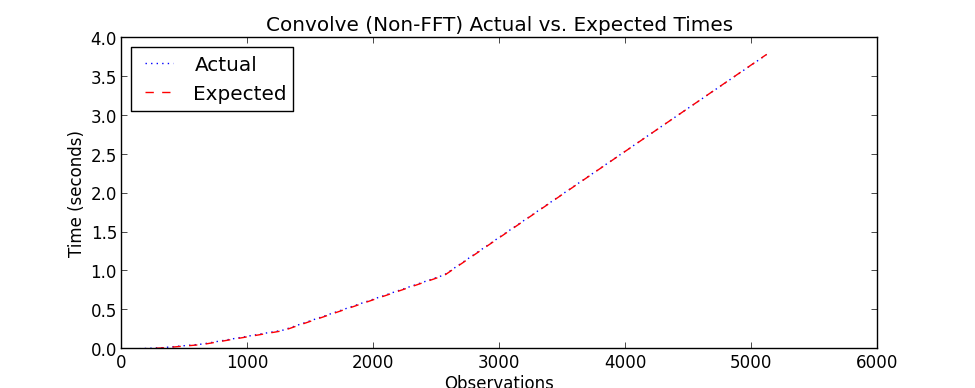
\includegraphics[width=6.5in]{./include/convolve_nonfft.png}
    \label{fig:convolve_nonfft}
    \caption{Non-FFT Actual vs. Expected Times}
\end{figure}\noindent
Figure~\ref{fig:convolve_nonfft} illustrates that the Non-FFT convolution times are as expected. It is shown that the actual times observed for the Non-FFT convolution, plus the \emph{Expected Times} calculated as previously stated. 

\begin{figure}[H]
    \centering
        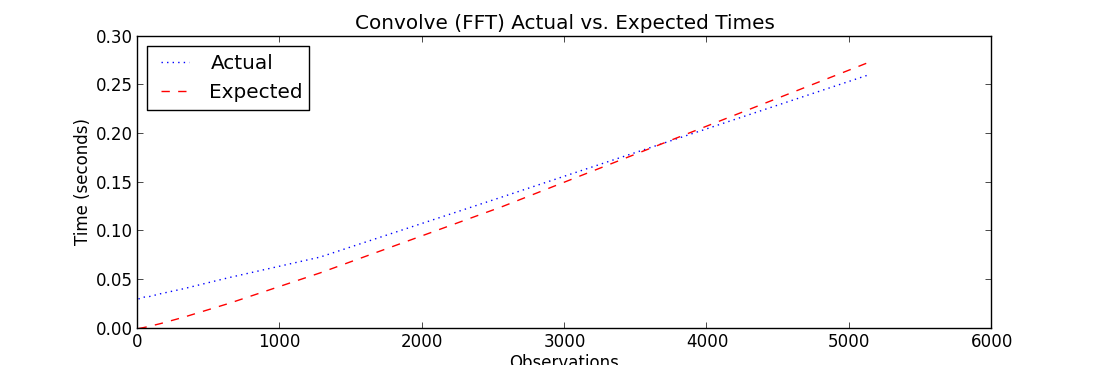
\includegraphics[width=6.5in]{./include/convolve_fft.png}
        \caption{FFT Actual vs. Expected Times}
        \label{fig:convolve_fft}
\end{figure}\noindent
Similarly, Figure~\ref{fig:convolve_fft} depicts that the FFT convolution also follows the expected trend. It is interesting to note that the plotted times do not go through the origin due to the computational overhead of these functions. However, it becomes obvious as n is large that the order is indeed $\mathcal{O}(n \log_2(n))$.

\begin{figure}[H]
    \centering
        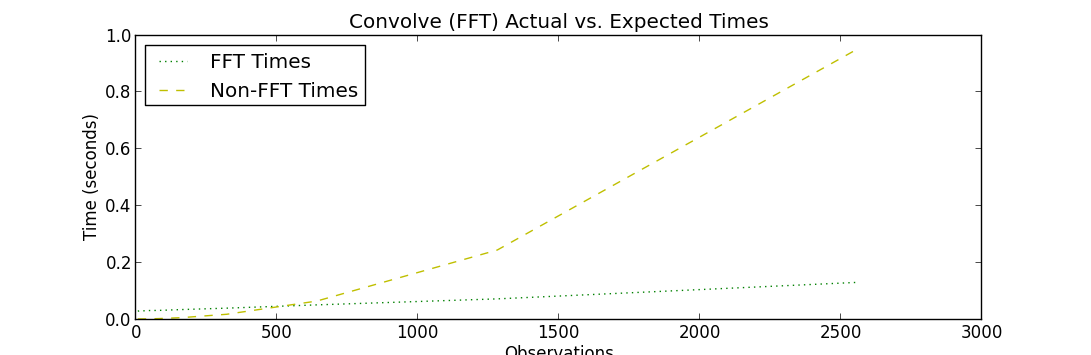
\includegraphics[width=6.5in]{./include/convolve_fft_vs_nonfft.png}
        \caption{Comparison of FFT vs Non-FFT Convolution}
        \label{fig:convolve_fft_vs_nonfft}
\end{figure}\noindent
Lastly, we examined under what conditions was the FFT faster than the Non-FFT. Figure~\ref{fig:convolve_fft_vs_nonfft} shows the two times plotted against each other. The reader should note that for small values of $n$, the Non-FFT convolution was actually faster. However, for large values of $n$, FFT convolution was significantly faster. 

% subsection results (end) 
	
	
\end{document}